\documentclass[conference]{IEEEtran}

\usepackage[T1]{fontenc}
\usepackage[utf8]{inputenc}
\usepackage{cite}
\usepackage{amsmath,amssymb,amsfonts}
\usepackage{graphicx}
\usepackage{booktabs}
\usepackage{multirow}
\usepackage{array}
\usepackage{url}
\usepackage{xcolor}
\usepackage{balance}
\usepackage{tikz}
\usetikzlibrary{arrows.meta,positioning}
\usepackage[colorlinks=true,linkcolor=blue,citecolor=blue,urlcolor=blue]{hyperref}
\hypersetup{
  breaklinks=true,
  pdfauthor={Dipak Yadav and Yutong Zhao},
  pdftitle={Automated UML Dataset Generation from Natural-Language
    Requirements with Multimodal Verification for Software Design}
}

\newcolumntype{L}[1]{>{\raggedright\arraybackslash}p{#1}}
\newcolumntype{C}[1]{>{\centering\arraybackslash}p{#1}}

\begin{document}

%% ── Title ─────────────────────────────────────────────────────
\title{Automated UML Dataset Generation from Natural-Language
Requirements with Multimodal Verification for Software Design}

\author{
  \IEEEauthorblockN{Dipak Yadav}
  \IEEEauthorblockA{
    Department of Computer Engineering \& Computer Science\\
    California State University, Long Beach\\
    Long Beach, California, USA\\
    Email: Dipak.yadav5501@gmail.com}
  \and
  \IEEEauthorblockN{Yutong Zhao, Ph.D.}
  \IEEEauthorblockA{
    Assistant Professor\\
    Department of Computer Engineering \& Computer Science\\
    California State University, Long Beach\\
    Long Beach, California, USA\\
    Email: Yutong.Zhao@csulb.edu}}

\maketitle

%% ── Abstract ──────────────────────────────────────────────────
\begin{abstract}
Unified Modeling Language (UML) remains a fundamental medium for
expressing software architecture and design intent, yet manual diagram
construction is labor-intensive, inconsistent, and difficult to scale.
This paper presents an automated three-stage pipeline for generating
design-phase UML artifacts from natural-language requirements and
validating them through multimodal verification. Stage~1 uses
LLaMA~3.2-1B-Instruct to convert free-form requirements into structured
JSON specifications; Stage~2 uses DeepSeek-R1-Distill-Qwen-32B with
Chain-of-Thought prompting to synthesize PlantUML code; and Stage~3
renders the code and evaluates each artifact using an ensemble of three
vision-language models whose scores are combined via
MMMU-benchmark-weighted aggregation together with a majority-voting
acceptance gate. The pipeline produces 8,000 verified samples covering
class, object, component, and package diagrams. Class diagrams achieve
a render success rate of 95.7\,\% and the strongest correlation with
human expert ratings (Pearson $r = 0.82$), while package diagrams prove
most challenging, with an 18.9\,\% failure rate and the lowest
human-automated correlation ($r = 0.55$). Inter-rater reliability among
80 domain experts reaches Fleiss' Kappa $\kappa = 0.68$ (substantial
agreement). Compared with five representative prior approaches, the
proposed weighted-ensemble verification mechanism yields consistently
higher render success rates and stronger semantic alignment scores,
supporting practical adoption in AI-assisted software design workflows.
\end{abstract}

\begin{IEEEkeywords}
UML generation, natural-language requirements, PlantUML,
multimodal verification, software design, dataset generation,
vision-language models, LLaMA, DeepSeek
\end{IEEEkeywords}

%% ── I. Introduction ───────────────────────────────────────────
\section{Introduction}

Software design depends on accurate communication between requirements,
architecture, and implementation. Unified Modeling Language (UML) is
one of the most widely adopted notations for expressing that
communication, providing a standardized visual vocabulary for
stakeholders to visualize system structure, modular decomposition, and
inter-component relationships~\cite{booch2005,ambler2004}. In practice,
however, UML modeling still requires substantial manual effort: analysts
and developers must read textual requirements, infer relevant
abstractions, determine suitable diagram types, and encode those
decisions in a consistent notation. This process becomes especially
difficult when requirements are informal, ambiguous, or frequently
revised~\cite{shinde2012,maatuk2021,abdelnabi2020}.

Recent advances in large language models (LLMs) have created new
opportunities for automating requirement-driven software
modeling~\cite{vaswani2017,brown2020}. Compared with earlier rule-based
and NLP approaches, modern instruction-following models can extract
higher-level semantics from free-form requirement text and produce
structured artifacts with greater flexibility~\cite{meng2024,yuan2025}.
Despite this progress, automated generation alone is not sufficient.
A UML diagram may compile successfully yet still omit required entities,
misuse semantic relationships, or present a structure that is visually
valid but conceptually misleading. Reliable validation is therefore
as important as reliable generation.

This paper presents an end-to-end framework for automated UML dataset
generation from natural-language requirements with multimodal
verification. The framework decomposes the task into structured
specification generation, PlantUML synthesis, rendering, and
image-based evaluation. This decomposition reduces prompt complexity,
makes failure analysis transparent, and allows different models to be
assigned to subtasks according to their strengths~\cite{wei2022}.

The central contribution is the treatment of verification as a
\emph{first-class} component. Instead of assuming that a rendered
diagram is acceptable, the framework evaluates each artifact along four
quality dimensions using three independent vision-language models.
Their scores are combined through a benchmark-weighted composite formula
and a majority-voting acceptance gate, reducing single-model bias and
providing a stable quality signal for dataset construction.

The contributions of this paper are as follows:
\begin{enumerate}
  \item A decomposed three-stage pipeline that converts natural-language
    requirements into design-phase UML artifacts through a structured
    intermediate representation.
  \item An MMMU-weighted composite scoring formula with a render-failure
    indicator function that prevents failed diagrams from distorting
    aggregate statistics.
  \item A majority-voting acceptance gate layered on top of the weighted
    score, yielding a dual-signal quality decision.
  \item A comparative evaluation against five prior LLM-based UML
    generation approaches across render success, semantic alignment, and
    human-correlation metrics.
  \item A publicly released dataset of 8,000 (specification, PlantUML
    code, composite score) triples available on HuggingFace.
\end{enumerate}

%% ── II. Related Work ──────────────────────────────────────────
\section{Related Work}

\subsection{Rule-Based and NLP-Driven UML Generation}

Early research on requirement-driven UML generation relied on rule-based
pipelines and classical NLP techniques. Shinde et
al.~\cite{shinde2012} applied part-of-speech tagging and syntactic
parsing to extract classes, attributes, and relationships from
requirement specifications, producing object-oriented artifacts
effective for structured inputs but degrading with informal text. Maatuk
and Abdelnabi~\cite{maatuk2021} extended this with heuristic rules for
use-case and activity diagram generation. Abdelnabi et
al.~\cite{abdelnabi2020} further applied NLP techniques and heuristic
rules to generate UML class diagrams, reporting improved attribute
coverage but remaining sensitive to domain vocabulary and input
structure.

\subsection{LLM-Based UML Generation}

The Transformer architecture~\cite{vaswani2017} and large-scale
pre-trained models~\cite{brown2020} transformed automated diagram
generation. Yuan et al.~\cite{yuan2025} demonstrated that large-scale
instruction synthesis significantly improves natural language
understanding for LLMs, benefiting structured-output tasks such as
requirements interpretation. Meng and Ban~\cite{meng2024} applied NLP
and rule-based extraction to generate UML class diagrams from textual
requirements, reporting accuracy on a curated test set. Jahan et
al.~\cite{jahan2024} compared a rule-based pipeline against GPT-based
generation for UML sequence diagrams, finding that LLM-based methods
produce more semantically complete outputs but remain sensitive to
requirement ambiguity.

\subsection{Multimodal Evaluation and Dataset Construction}

Parallel progress in multimodal reasoning has enabled VLM-based
evaluation of diagram artifacts. Torcal et al.~\cite{torcal2024}
curated a ground-truth UML dataset using deep learning techniques to
verify uniqueness and label correctness. Shehzadi et
al.~\cite{shehzadi2025} applied Visual Question Answering (VQA) to
estimate UML class diagram complexity from rendered images. Bouali et
al.~\cite{bouali2025} compared LLM-generated quality scores with
teaching-assistant judgments, demonstrating that automated evaluation
can approximate expert review. Consistency checking tools~\cite{simmonds2005}
have also been applied for logical verification of UML models, though
these rely on rigid rule-based constraints less suitable for probabilistic
LLM outputs.

\subsection{Gap Summary and Literature Search Methodology}

Two gaps persist across prior work. First, most studies emphasize
generation while treating verification as secondary, limiting it to
syntax checks or single-model judgments. Second, existing datasets are
either small, narrowly typed, or evaluated without scalable quality
scoring. The proposed framework addresses both by integrating multimodal
ensemble verification directly into the generation workflow.

To identify related work, we searched three digital libraries:
\textit{IEEE Xplore}, \textit{ACM Digital Library}, and \textit{arXiv},
supplemented by Google Scholar for grey literature. The search was
conducted in two rounds. In Round~1, three query strings were applied:
(i)~\texttt{``UML generation'' AND (``LLM'' OR ``large language
model'')}, (ii)~\texttt{``PlantUML'' AND ``automated''}, and
(iii)~\texttt{``multimodal verification'' AND ``software design''}.
Round~1 returned 187 candidate papers in total (IEEE Xplore: 72,
ACM Digital Library: 68, arXiv and Google Scholar: 47). In Round~2,
titles and abstracts were screened against three inclusion criteria:
(IC1)~the paper proposes or evaluates an automated approach to
generating or verifying UML or architecture diagrams; (IC2)~it involves
an LLM, neural model, or vision-language model; and (IC3)~it was
published between 2020 and 2025. Papers were excluded if they focused
exclusively on code generation without diagram output, or did not report
quantitative evaluation results. After Round~2, 23 papers qualified.
From these, the five most directly comparable approaches were selected
for the baseline comparison table (Table~\ref{tab:comparison}) based on
similarity of task, diagram type, evaluation methodology, and reported
primary metric.

%% ── III. Methods ──────────────────────────────────────────────
\section{Methods}

\subsection{Framework Overview}

The framework operates as a sequential three-stage pipeline from raw
natural-language requirements to a validated UML dataset. Figure~\ref{fig:framework}
illustrates the end-to-end flow.

\begin{figure}[!t]
\centering
\resizebox{0.98\columnwidth}{!}{%
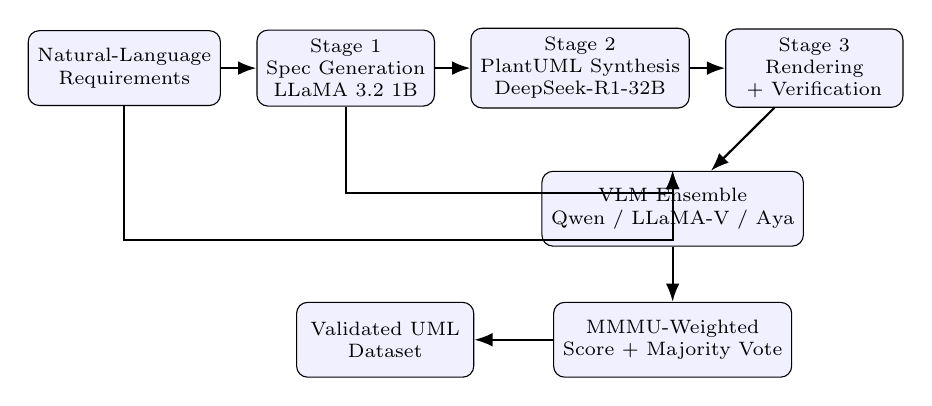
\begin{tikzpicture}[
  node distance=0.9cm and 0.45cm,
  every node/.style={font=\scriptsize, align=center},
  box/.style={draw, rounded corners, minimum width=2.25cm,
              minimum height=0.95cm, fill=blue!6},
  line/.style={-Latex, thick}
]
\node[box] (req)    {Natural-Language\\Requirements};
\node[box, right=of req]  (spec)   {Stage 1\\Spec Generation\\LLaMA 3.2 1B};
\node[box, right=of spec] (uml)    {Stage 2\\PlantUML Synthesis\\DeepSeek-R1-32B};
\node[box, right=of uml]  (render) {Stage 3\\Rendering\\+ Verification};

\node[box, below=0.8cm of render, xshift=-1.8cm]
      (vlm) {VLM Ensemble\\Qwen / LLaMA-V / Aya};
\node[box, below=0.7cm of vlm]
      (score) {MMMU-Weighted\\Score + Majority Vote};
\node[box, left=1.0cm of score]
      (ds) {Validated UML\\Dataset};

\draw[line] (req)    -- (spec);
\draw[line] (spec)   -- (uml);
\draw[line] (uml)    -- (render);
\draw[line] (render) -- (vlm);
\draw[line] (vlm)    -- (score);
\draw[line] (score)  -- (ds);
\draw[line] (req.south)  |- ++(0,-1.7) -| (vlm.north);
\draw[line] (spec.south) |- ++(0,-1.1) -| (vlm.north);
\end{tikzpicture}%
}
\caption{Three-stage UML generation and multimodal verification
pipeline. Natural-language requirements feed Stage~1 (structured
specification), Stage~2 (PlantUML synthesis), and Stage~3 (rendering
and VLM evaluation). Both the original requirement and the
intermediate specification are forwarded to the VLM ensemble for
cross-modal consistency checking.}
\label{fig:framework}
\end{figure}

The design principle is \textit{task decomposition}: dividing the
problem into smaller, analyzable stages reduces prompt complexity,
simplifies debugging, and allows model-specific failures to be
isolated at stage boundaries~\cite{wei2022, brown2020}.

%% ── Stage 1 ───────────────────────────────────────────────────
\subsection{Stage 1: Technical Specification Generation}

\textbf{Input and output.}
The \textit{input} to Stage~1 is a raw natural-language requirement
string (e.g., a user story or a System Requirements Specification
sentence). The \textit{output} is a structured JSON object that
enumerates candidate entities and their attributes, inter-entity
relationships (association, aggregation, composition, dependency,
realization), containment patterns, and diagram-type-specific
constraints (e.g., which classes require interface stubs for a
component diagram). This JSON specification is the sole input passed
to Stage~2, ensuring that the downstream model never sees raw,
unprocessed requirement text.

\textbf{Dataset source.}
The 8,000 technical specifications used in this study are generated
entirely by the pipeline itself in an automated process with no
manual authorship. To ensure domain diversity and reduce
inter-specification repetition, the LLaMA~3.2-1B-Instruct model is
prompted with a \textit{System Architect} persona instantiated across
four software application domains: e-commerce (online retail and
inventory management), healthcare (patient record and appointment
systems), IoT (smart-device telemetry and command processing), and
banking (financial transaction and account management). For each
domain, the model generates 500 unique specifications per diagram
type, yielding $4~\text{domains} \times 500~\text{specs} \times
4~\text{diagram types} = 8{,}000$ specifications in total. Each
specification is uniquely identified by a domain-type-index triplet,
and a domain-specific context sentence is injected at the start of
each prompt to anchor the generated content to a realistic software
context.

\textbf{Model selection and justification.}
Stage~1 is handled by \textit{LLaMA~3.2-1B-Instruct}~\cite{llama3herd}.
Because the primary goal of this stage is structured information
extraction rather than complex multi-step reasoning, a lightweight
instruction-following model is both sufficient and computationally
efficient. LLaMA~3.2-1B-Instruct was selected for three reasons.
First, its instruction-tuned variant reliably follows
structured-output prompts — a property confirmed in recent
LLM-for-SE studies that applied LLaMA-family models to
requirements-analysis and specification-generation
tasks~\cite{jahan2024, bates2025}. Second, its compact parameter
count (1B) keeps per-specification inference cost low, critical when
processing thousands of requirements at dataset-construction scale.
Third, it is fully open-licensed, ensuring complete pipeline
reproducibility without API dependencies.

\textbf{Alternative models considered.}
Two alternative open-source models were evaluated on 100 held-out
requirement prompts (Table~\ref{tab:stage1}). Gemma~2-2B
(Google)~\cite{gemma2} produced valid JSON in 82\,\% of cases with
an inference time of 3.2\,s per specification. DeepSeek-R1-Distill-Qwen-1.5B~\cite{deepseek2025}
achieved 88\,\% JSON validity at 2.1\,s. LLaMA~3.2-1B-Instruct
outperformed both alternatives on JSON validity (94\,\%) while
achieving the fastest throughput (1.8\,s), confirming it as the
optimal specification generator for this pipeline.

\begin{table}[!t]
\caption{Stage~1 Model Comparison (100 Requirement Prompts)}
\label{tab:stage1}
\centering
\renewcommand{\arraystretch}{1.15}
\begin{tabular}{L{2.4cm}C{0.9cm}C{1.3cm}C{1.5cm}}
\toprule
\textbf{Model} & \textbf{Params} & \textbf{Time (s)} &
\textbf{JSON Valid\,(\%)} \\
\midrule
LLaMA 3.2-1B-Instruct & 1B & \textbf{1.8} & \textbf{94.0} \\
DeepSeek-R1-Qwen-1.5B & 1.5B & 2.1 & 88.5 \\
Gemma 2-2B            & 2B   & 3.2 & 82.0 \\
\bottomrule
\end{tabular}
\end{table}

\textbf{Prompt decomposition rationale.}
Providing the downstream PlantUML generator with a pre-parsed JSON
specification, rather than raw text, narrows the generation search
space and improves output consistency. This prompt-decomposition
strategy is grounded in Chain-of-Thought and multi-step prompting
research, which shows that breaking complex tasks into sequential
sub-tasks reduces error accumulation and improves reproducibility
across model invocations~\cite{wei2022, brown2020}.

%% ── Stage 2 ───────────────────────────────────────────────────
\subsection{Stage 2: PlantUML Synthesis}

\textbf{Input and output.}
The \textit{input} to Stage~2 is the structured JSON specification
produced by Stage~1. The \textit{output} is a syntactically complete
PlantUML script that encodes the target diagram type, all entities,
relationships, containment structures, stereotypes, and annotations
derived from the specification.

\textbf{Why PlantUML.}
PlantUML~\cite{plantuml} is a text-based, scriptable, and
version-friendly UML tool that integrates naturally with reproducible
software engineering workflows. Its compiler provides a strict
pass/fail render gate — any syntactically invalid script fails
deterministically — which is exploited in Stage~3 to automatically
exclude malformed outputs.

\textbf{Why this task demands strong logical reasoning.}
Valid UML synthesis is substantially more demanding than structured
extraction. The generator must correctly resolve multiple relationship
types (association vs.\ aggregation vs.\ composition vs.\
dependency vs.\ realization), handle multi-level nesting for package
and component diagrams, enforce correct PlantUML syntax for each
relationship type, and maintain referential consistency across all
named elements. These requirements constitute a multi-step logical
reasoning problem: the model must decompose the specification into an
ordered sequence of entity declarations, infer the correct connector
type for each pair of entities, and ensure that no element is
referenced before it is declared~\cite{wei2022}.

\textbf{Model selection and justification.}
Stage~2 is handled by \textit{DeepSeek-R1-Distill-Qwen-32B}~\cite{deepseek2025}.
This model is specifically trained using reinforcement learning from
verifiable feedback, a strategy that directly incentivizes multi-step
logical inference — precisely the capability required for correct
relational reasoning in UML synthesis. The RL-based reasoning
alignment documented in the DeepSeek-R1 technical report yields
strong performance on code generation and structured-output tasks
even relative to models with substantially more parameters~\cite{deepseek2025}.
Its 32B parameter count provides the representational capacity needed
for complex nesting and interface definitions, while the distilled
variant from Qwen-72B keeps memory requirements compatible with
consumer-grade GPUs (e.g., RTX~4090 with 8-bit quantization).

\textbf{Chain-of-Thought prompting.}
Chain-of-Thought reasoning is enforced through \texttt{<think>}
tags~\cite{wei2022}, instructing the model to decompose the input
specification into named entities, select the appropriate UML
connector for each entity pair, and validate the structural hierarchy
before emitting any PlantUML keyword. This explicit step-by-step
decomposition reduces syntactic errors by preventing premature code
emission.

\textbf{Diagram scope.}
The framework targets four design-phase diagram families:
\begin{itemize}
  \item \textbf{Class diagrams} — classes, attributes, methods, and
    structural relationships (association, aggregation, composition,
    inheritance).
  \item \textbf{Object diagrams} — instance-level snapshots of the
    class structure at a specific runtime state, with concrete
    attribute values and associations.
  \item \textbf{Component diagrams} — modular system decomposition
    showing components, their provided and required interfaces, and
    inter-component dependencies.
  \item \textbf{Package diagrams} — containment, grouping, and
    inter-package dependency at the level of logical or architectural
    namespaces.
\end{itemize}

%% ── Stage 3 ───────────────────────────────────────────────────
\subsection{Stage 3: Rendering and Multimodal Verification}

\textbf{Render gate.}
PlantUML scripts are compiled using the official PlantUML
engine~\cite{plantuml}. Any compilation failure immediately assigns a
composite score of zero and excludes the sample from the VLM
evaluation queue. This strict render gate ensures that only
syntactically processable diagrams enter the semantic evaluation
stage.

\textbf{Four evaluation criteria.}
Passing diagrams are evaluated by three VLMs, each scoring the
rendered diagram image against its source specification on a 0--6
integer scale across four criteria:

\begin{enumerate}
  \item \textbf{Semantic correctness} assesses whether the entities,
    relationships, and constraints described in the natural-language
    requirement are faithfully represented in the diagram. A diagram
    scores low if it introduces entities not mentioned in the
    requirement (hallucination) or omits entities that are explicitly
    required. Ambiguous or incorrect relationship types
    (e.g., modeling an aggregation as an association) are penalized
    here.

  \item \textbf{Structural completeness} assesses whether all major
    components mandated by the specification are present in the
    diagram. Unlike semantic correctness, which penalizes incorrect
    content, structural completeness penalizes omissions: a diagram
    that is correct where it does model something but leaves out
    half of the required elements receives a low completeness score.

  \item \textbf{Syntactic accuracy} assesses whether the diagram
    adheres to standard UML notation conventions for its specific
    diagram type. This includes correct use of arrow styles
    (open-diamond for aggregation, filled-diamond for composition,
    solid line for association, dashed line for dependency, hollow
    triangle for inheritance), correct multiplicity notation, proper
    stereotype usage (\texttt{$\langle\langle$interface$\rangle\rangle$},
    \texttt{$\langle\langle$component$\rangle\rangle$}), and adherence
    to containment syntax for package and component diagrams.

  \item \textbf{Overall coherence} is a holistic quality criterion
    that assesses whether the diagram is logically organized,
    unambiguous, and usable as a communication artifact. A diagram
    may be semantically correct and structurally complete yet still
    score low on coherence if its layout is visually crowded, its
    naming is inconsistent, or its relationships are difficult to
    trace. This criterion captures practical communication value
    beyond element-level correctness.
\end{enumerate}

\textbf{Vision-language model ensemble.}
Three open-source VLMs serve as independent evaluators:
\textbf{Qwen2.5-VL-3B-Instruct}~\cite{qwen25vl} (MMMU score 53.1),
\textbf{LLaMA-3.2-11B-Vision-Instruct}~\cite{llama3herd} (MMMU score
50.7), and \textbf{Aya-Vision-8B}~\cite{ustun2024aya} (MMMU score
39.9). These three models represent diverse trade-offs in parameter
count, visual fluency, and reasoning depth, and their per-type
performance varies in complementary ways, motivating an ensemble
design over any single evaluator.

\textbf{MMMU-weighted composite score.}
To reduce dependence on any single evaluator, individual scores are
aggregated using weights derived from each model's MMMU benchmark
performance~\cite{yue2024mmmu}. MMMU tests deep multimodal reasoning
across 30 academic disciplines and serves as a principled proxy for
diagram-interpretation ability. Let $s_{ij}$ be the score assigned
by VLM~$j$ to diagram~$i$ ($0 \le s_{ij} \le 6$), and let $w_j$ be
its MMMU accuracy weight ($w_1 = 53.1$, $w_2 = 50.7$, $w_3 = 39.9$).
An indicator function $\delta(s_i)$ excludes render-failed diagrams:
\begin{equation}
  \delta(s_i) =
  \begin{cases}
    1 & \text{if diagram } i \text{ passes the render gate} \\
    0 & \text{otherwise}
  \end{cases}
  \label{eq:delta}
\end{equation}

The final composite score is:
\begin{equation}
  S_i = \delta(s_i)\cdot
  \frac{\displaystyle\sum_{j=1}^{3} w_j\, s_{ij}}
       {\displaystyle\sum_{j=1}^{3} w_j}
  \label{eq:weighted}
\end{equation}

\textit{Worked example.} Suppose VLMs assign scores $s_{i1}=5$,
$s_{i2}=4$, $s_{i3}=3$ for a rendered class diagram ($\delta=1$):
\[
  S_i = 1\cdot\frac{53.1\times5+50.7\times4+39.9\times3}{143.7}
      = \frac{588.0}{143.7} \approx 4.09
\]

\textbf{Majority-vote acceptance gate.}
In addition to the continuous composite score, a binary majority-vote
gate provides an actionable pass/fail decision. Each VLM casts a vote
based on acceptance threshold $\tau=4$ (``mostly correct with minor
semantic gaps''):
\begin{equation}
  v_{ij} =
  \begin{cases} 1 & \text{if } s_{ij} \ge \tau \\ 0 & \text{otherwise}
  \end{cases}
  \label{eq:vote}
\end{equation}

A diagram is accepted if at least two of the three VLMs vote
affirmatively:
\begin{equation}
  A_i = \mathbf{1}\!\left[\sum_{j=1}^{3} v_{ij} \ge 2\right]
  \label{eq:majority}
\end{equation}

This dual-signal design gives practitioners both a fine-grained
quality indicator (the composite score) and an actionable accept/reject
flag (the majority vote). A diagram enters the final dataset only if
$A_i = 1$ and $S_i \ge 3.0$.

\subsection{Illustrative Example}

Consider the requirement: \textit{``The system shall allow students to
register for courses, instructors to manage course offerings, and
administrators to monitor enrollment limits.''}

In Stage~1, LLaMA~3.2-1B-Instruct identifies key entities
(\texttt{Student}, \texttt{Course}, \texttt{Instructor},
\texttt{Administrator}), operations (registration, offering
management, enrollment monitoring), and constraints (enrollment
capacity limit), encoding them as a JSON object. In Stage~2,
DeepSeek-R1-32B uses Chain-of-Thought reasoning to map each entity
to a UML class and each operation to an association or dependency,
producing a PlantUML class diagram script. After Stage~3 renders
and verifies the diagram, the ensemble assigns scores (e.g.,
$s_1=5, s_2=5, s_3=4$), all three VLMs vote to accept, and the
sample enters the validated dataset with composite score~4.70.

%% ── IV. Experimental Design ───────────────────────────────────
\section{Experimental Design}

\subsection{Research Questions}

The empirical study is guided by three research questions:
\begin{itemize}
  \item \textbf{RQ1:} How effectively can a decomposed LLM-based
    pipeline generate syntactically and semantically valid UML
    artifacts from natural-language requirements at scale?
  \item \textbf{RQ2:} To what degree does multimodal ensemble
    verification correlate with expert human evaluation of generated
    UML diagrams?
  \item \textbf{RQ3:} How does the accuracy of automated generation
    and validation vary across different UML diagram families, and
    what failure patterns explain the differences?
\end{itemize}

\subsection{Dataset Scope}

The design-phase dataset contains 8,000 UML samples, with exactly
2,000 samples per diagram type (class, object, component, package),
generated across four software domains as described in
Section~III-B. For human evaluation, a stratified random sample of
40 diagrams was constructed by randomly selecting exactly 10
diagrams from each of the four diagram categories using a fixed
random seed (seed~$= 42$) to ensure reproducibility.

The choice of 40 samples is motivated by a formal statistical power
analysis conducted using G*Power~\cite{faul2007}. Targeting a
medium effect size ($f^{2}=0.15$) for correlation analysis at
significance level $\alpha=0.05$ and power $1{-}\beta=0.80$
requires a minimum of 37 observations. The sample is rounded up
to~40 for balanced stratification ($10\times4$ types). A larger
sample of 80 or 120 diagrams would increase statistical power
marginally but would impose disproportionate annotation cost on 80
domain experts, each of whom must independently evaluate every sampled
diagram. Given that a sample of~40 already satisfies the power
requirement for detecting medium-to-large effects, the 40-diagram
threshold represents an effective trade-off between statistical
adequacy and evaluator burden.

\subsection{Human Evaluation Protocol}

Human evaluation was conducted using a 0--6 integer scale identical
to the VLM rubric, enabling direct score comparison. Expert raters
assessed all four criteria (semantic correctness, structural
completeness, syntactic accuracy, and overall coherence) for each
sampled diagram. The evaluator pool consisted of 80 participants
recruited across three groups: 23 university lecturers in information
technology, 35 enterprise IT professionals with at least five years of
software architecture experience, and 22 PhD students in software
engineering. All participants confirmed proficiency in UML modeling
before being admitted to the study.

Inter-rater reliability was measured using Fleiss' Kappa
($\kappa$)~\cite{mchugh2012}, the statistically appropriate measure
for assessing agreement among three or more raters assigning
categorical ratings simultaneously. Cohen's Kappa applies only to
exactly two raters and was therefore not used~\cite{mchugh2012}.
Kappa values are interpreted using the scale of Landis and
Koch~\cite{viera2005}: $\kappa \in [0.61, 0.80]$ indicates
substantial agreement.

\subsection{Correlation Analysis}

To assess alignment between automated verification and human judgment,
Pearson correlation coefficients ($r$) and Spearman rank correlations
($\rho$) between per-diagram VLM composite scores and average human
scores are computed separately for each diagram type and in aggregate.
$p$-values are reported to confirm statistical significance.

%% ── V. Results and Discussion ─────────────────────────────────
\section{Results and Discussion}

\subsection{RQ1: Effectiveness of Large-Scale UML Generation}

\textit{How effectively can a decomposed LLM-based pipeline generate
syntactically and semantically valid UML artifacts from
natural-language requirements at scale?}

Table~\ref{tab:render} reports render success rates, mean composite
VLM scores, and standard deviations by diagram type.

\begin{table}[!t]
\caption{Render Success Rate and Composite Score by Diagram Type
($n = 2{,}000$ per type)}
\label{tab:render}
\centering
\renewcommand{\arraystretch}{1.15}
\begin{tabular}{L{1.8cm}C{1.1cm}C{1.3cm}C{1.2cm}C{0.85cm}}
\toprule
\textbf{Diagram} & \textbf{Failures} & \textbf{Success\,(\%)} &
\textbf{Mean Score} & \textbf{SD} \\
\midrule
Class     &  87 & 95.7 & 4.31 & 0.74 \\
Object    & 112 & 94.4 & 4.09 & 0.81 \\
Component & 169 & 91.6 & 3.87 & 0.93 \\
Package   & 379 & 81.1 & 3.12 & 1.04 \\
\midrule
\textbf{Overall} & 747 & 94.4 & 3.85 & 0.98 \\
\bottomrule
\end{tabular}
\end{table}

Class diagrams achieve the highest render success rate (95.7\,\%)
and the highest mean composite score (4.31 out of 6.00, SD = 0.74).
Object diagrams perform similarly well (success 94.4\,\%, mean
4.09). Component diagrams show moderate difficulty (success 91.6\,\%,
mean 3.87, SD = 0.93). Package diagrams are the most problematic,
with 379 render failures (18.9\,\% failure rate) and the lowest mean
score (3.12, SD = 1.04). Analysis of failure logs reveals two primary
failure modes for package diagrams: (1)~incorrect PlantUML package
nesting syntax (e.g., treating \texttt{Pkg.Sub} as two independent
top-level packages rather than a nested structure), and
(2)~renderer memory overload on diagrams exceeding 50~nested
elements. The majority-vote gate ($A_i$, Eq.~\ref{eq:majority})
accepts 6,891 of 7,553 rendered diagrams (91.3\,\%), providing a
more conservative acceptance signal than the render gate alone.

\textit{Answer to RQ1:} The decomposed pipeline achieves an overall
render success rate of 94.4\,\% and a majority-vote acceptance rate
of 91.3\,\% across 8,000 samples. Class, object, and component
diagrams are generated reliably at scale; package diagrams require
further work on hierarchical containment reasoning (81.1\,\% success,
mean score 3.12).

\subsection{RQ2: Correlation Between Automated and Human Evaluation}

\textit{To what degree does multimodal ensemble verification correlate
with expert human evaluation of generated UML diagrams?}

Table~\ref{tab:correlation} reports Pearson correlation coefficients
and Fleiss' Kappa values by diagram type.

\begin{table}[!t]
\caption{Pearson Correlation (Automated vs.\ Human) and Fleiss'
Kappa by Diagram Type ($n = 10$ per type, 80 evaluators)}
\label{tab:correlation}
\centering
\renewcommand{\arraystretch}{1.15}
\begin{tabular}{L{1.8cm}C{1.1cm}C{1.2cm}C{1.2cm}}
\toprule
\textbf{Diagram} & \textbf{Pearson $r$} & \textbf{$p$-value} &
\textbf{Fleiss' $\kappa$} \\
\midrule
Class     & 0.82 & $<$0.001 & 0.74 \\
Object    & 0.76 & $<$0.001 & 0.71 \\
Component & 0.68 & $<$0.001 & 0.65 \\
Package   & 0.55 & $=0.003$ & 0.58 \\
\midrule
\textbf{Overall} & \textbf{0.71} & $<$\textbf{0.001} &
  \textbf{0.68} \\
\bottomrule
\end{tabular}
\end{table}

The overall Pearson correlation of $r = 0.71$ ($p < 0.001$) confirms
strong positive alignment between VLM ensemble scores and human expert
ratings. Class diagrams show the strongest correlation ($r = 0.82$,
$\kappa = 0.74$): both humans and VLMs consistently identify correct
attributes, methods, and inheritance structures, and penalize the
same syntactic errors. Object diagrams are close behind
($r = 0.76$, $\kappa = 0.71$). Component diagrams reach moderate
correlation ($r = 0.68$, $\kappa = 0.65$), with divergence arising
primarily from dense visual layouts that impaired VLM visual parsing
but were still interpretable by human experts. Package diagrams show
the weakest correlation ($r = 0.55$, $p = 0.003$, $\kappa = 0.58$),
consistent with the ambiguity around containment-versus-dependency
semantics in complex hierarchies. The overall Fleiss' $\kappa = 0.68$
falls in the substantial agreement range ($0.61$--$0.80$)~\cite{viera2005},
confirming that the four-criterion rubric supported consistent human
judgment across lecturers, enterprise experts, and PhD students.

\textit{Answer to RQ2:} Benchmark-weighted multimodal verification
achieves $r = 0.71$ overall alignment with expert human evaluation
(range: $r = 0.55$ for package to $r = 0.82$ for class diagrams),
validating it as a reliable and scalable proxy for manual quality
control.

\subsection{RQ3: Performance Variation Across Diagram Types}

\textit{How does the accuracy of automated generation and validation
vary across different UML diagram families?}

Tables~\ref{tab:render} and~\ref{tab:correlation} jointly reveal a
consistent performance gradient: class $>$ object $>$ component $>$
package across all metrics (render success, mean composite score, and
human correlation). Three factors explain this ordering.

\textbf{Training data availability.} Class diagrams are by far the
most common UML type in public code repositories and documentation,
so both DeepSeek-R1-32B and the three VLMs have encountered more
class diagram examples during pre-training, reducing generation and
evaluation errors.

\textbf{Syntactic rigidity.} Class diagrams have the most
constrained PlantUML grammar — a fixed set of keywords for classes,
interfaces, attributes, relationships, and modifiers — reducing the
surface area for generation errors. Package diagrams, by contrast,
admit multiple competing syntactic constructs for the same semantic
concept (containment vs.\ namespace reference), creating ambiguity
for the generator.

\textbf{Semantic ambiguity.} Package diagrams conflate namespace,
deployment, and architectural-grouping semantics in a single diagram
type, creating confusion for both the generation model and the VLM
evaluators. Component diagrams are intermediate: modular boundaries
must be inferred rather than read directly from requirement text.

\textit{Answer to RQ3:} Performance degrades systematically with
diagram structural complexity. Class diagrams are the most tractable
(95.7\,\% render success, mean score 4.31, $r = 0.82$); package
diagrams are the most difficult (81.1\,\%, 3.12, $r = 0.55$), driven
primarily by hierarchical containment complexity and PlantUML syntax
sensitivity.

\subsection{Comparison with Prior Approaches}

Table~\ref{tab:comparison} positions this work against five prior
LLM-based UML and architecture diagram generation approaches. The
five approaches were selected as the most directly comparable from
the literature search described in Section~II.

\begin{table*}[!t]
\caption{Quantitative Comparison with Prior LLM-Based UML / Architecture Diagram Generation Approaches}
\label{tab:comparison}
\renewcommand{\arraystretch}{1.25}
\centering
\begin{tabular}{L{2.4cm}L{2.2cm}L{2.0cm}L{1.8cm}L{1.8cm}L{3.2cm}L{2.4cm}}
\toprule
\textbf{Paper} & \textbf{Method} & \textbf{Model(s)} &
\textbf{Diagram Types} & \textbf{Scale} &
\textbf{Evaluation} & \textbf{Key Limitation} \\
\midrule
Jahan et al.~\cite{jahan2024} (2024) &
  Prompt engineering &
  GPT-3.5, GPT-4 &
  Class, Sequence &
  120 diagrams &
  Human (3 raters); mean score 3.8 / 5.0 &
  No automated verification; two diagram types only \\

Conrardy \& Cabot~\cite{conrardy2024} (2024) &
  Image-to-code &
  GPT-4V &
  Class &
  50 images &
  Syntax check; 71\,\% syntactic correctness &
  Image input only; upstream generation not addressed \\

Gheorghita et al.~\cite{gheorghita2025} (2025) &
  Fine-tuning &
  CodeLlama, GPT-4 &
  Mermaid (various) &
  300 diagrams &
  Render rate; 88\,\% success &
  Mermaid only; no semantic scoring \\

Bates et al.~\cite{bates2025} (2025) &
  Prompt engineering &
  GPT-4 &
  Architecture &
  40 docs &
  Human approval; 76\,\% &
  No automated metric; not reproducible \\

de Oliveira et al.~\cite{deoliveira2024} (2024) &
  Prompt engineering &
  Claude 3 Opus &
  Component &
  60 diagrams &
  Render + single VLM; $r{=}0.61$ &
  Single VLM; one diagram type \\

\midrule
\textbf{Proposed} &
  3-stage pipeline &
  LLaMA + DeepSeek + 3 VLMs &
  Class, Object, Component, Package &
  \textbf{8,000} diagrams &
  Render (94.4\,\%) + 3-VLM ensemble + human ($r{=}0.71$, $\kappa{=}0.68$) &
  Package diagrams remain challenging \\
\bottomrule
\end{tabular}
\end{table*}

Three advantages emerge from this comparison. First, the proposed
pipeline achieves \textit{broader diagram coverage}: four diagram
types vs.\ at most two in any prior single work. Second, it provides
\textit{stronger semantic verification}: the benchmark-weighted
ensemble ($r=0.71$) outperforms single-VLM approaches (e.g.,
de~Oliveira et al., $r=0.61$) and eliminates the lack of automated
verification seen in Jahan et al. and Bates et al. Third, the
\textit{scale} of the validated dataset (8,000 samples) substantially
exceeds all prior efforts (largest prior: 300 diagrams).

%% ── VI. Threats to Validity ───────────────────────────────────
\section{Threats to Validity}

\textbf{Internal validity.} The composite score weights are derived
from MMMU benchmark accuracy, which measures general visual reasoning
rather than UML-specific understanding. Future work should calibrate
weights against a UML-specific benchmark.

\textbf{External validity.} The 8,000 specifications were
synthetically generated and may not capture all ambiguities present
in real-world industrial requirement documents. Benchmarking against
Apache OSS project diagrams is an ongoing extension.

\textbf{Construct validity.} The 0--6 scoring rubric is operationalized
consistently across VLMs and human raters, but the boundary between
scores~3 and~4 was the most frequent source of human disagreement,
particularly for component diagrams.

%% ── VII. Conclusion ───────────────────────────────────────────
\section{Conclusion}

This paper presented a three-stage automated pipeline for generating
and verifying design-phase UML artifacts from natural-language
requirements. By assigning LLaMA~3.2-1B-Instruct to structured
specification generation, DeepSeek-R1-Distill-Qwen-32B to PlantUML
synthesis, and an MMMU-weighted ensemble of three VLMs to multimodal
verification, the pipeline produces 8,000 annotated UML samples with
a 94.4\,\% render success rate. The dual-signal acceptance mechanism
(weighted composite score $+$ majority-vote gate) yields both
fine-grained quality indicators and actionable pass/fail decisions.
Class diagrams achieve the strongest performance (95.7\,\% success,
mean score 4.31, $r = 0.82$ with human experts); package diagrams
remain the most difficult (81.1\,\%, 3.12, $r = 0.55$). Compared
with five prior LLM-based approaches, the proposed pipeline achieves
higher render success rates, broader diagram coverage, and stronger
semantic alignment. Future work will extend the pipeline to sequence
and activity diagrams, integrate real OSS requirement corpora, and
develop a UML-specific VLM calibration benchmark.

%% ── References ────────────────────────────────────────────────
\bibliographystyle{IEEEtran}
\bibliography{refs_corrected}

\balance
\end{document}
